% ==========================================
% SEÇÃO 1: INTRODUÇÃO E FÍSICA DA LUZ
% ==========================================
\section{Introdução}

\begin{frame}{Percepção Humana}
    \begin{columns}
        \begin{column}{0.45\textwidth}
            \begin{itemize}
                \item \textbf{Fotorreceptores na Retina:}
                \begin{itemize}
                    \item Bastonetes ($\approx$ 125 milhões).
                    \item Cones ($\approx$ 6 a 7 milhões).
                \end{itemize}
                \vspace{0.3cm}
                \item \textbf{Teoria Tricromática:}
                \begin{itemize}
                    \item Azul.
                    \item Verde.
                    \item Vermelho/Amarelo.
                \end{itemize}
            \end{itemize}
        \end{column}
        
        \begin{column}{0.55\textwidth}
            \begin{figure}
                \centering
                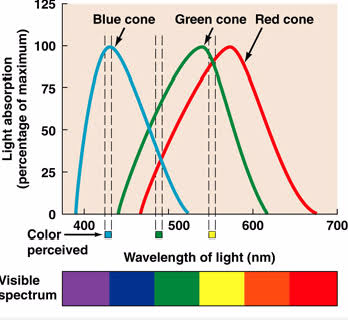
\includegraphics[width=0.75\textwidth]{images/curvas_sensibilidade_cones.jpg}
                \caption{Curvas de resposta espectral dos cones S, M e L.}
            \end{figure}
        \end{column}
    \end{columns}

    \note{
        A retina funciona com base em dois tipos de receptores:

        \begin{enumerate}
            \item \textbf{Bastonetes ($\approx$ 125 milhões):} São sensores de alta sensibilidade, mas monocromáticos. Eles não detectam cor, apenas intensidade luminosa. É a nossa visão noturna.
            
            \item \textbf{Cones ($\approx$ 6 a 7 milhões):} São os sensores responsáveis pela cor, mas que só funcionam bem com bastante luz. Note que nós temos muito menos sensores de cor do que de brilho.
        \end{enumerate}
        
        O gráfico ilustra a Teoria Tricromática, que é a base para a existência do RGB nos computadores. Nós não temos um cone para cada cor existente; a gente tem três tipos de cones (curtos: detectam azul. médios: detectam verde. longos: detectam vermelho/amarelo.), e o cérebro faz uma média ponderada dos sinais recebidos por eles.
    }
\end{frame}

\begin{frame}{Colorimetria}
    \begin{columns}
        \begin{column}{0.45\textwidth}
            \begin{figure}[H]
                \centering
                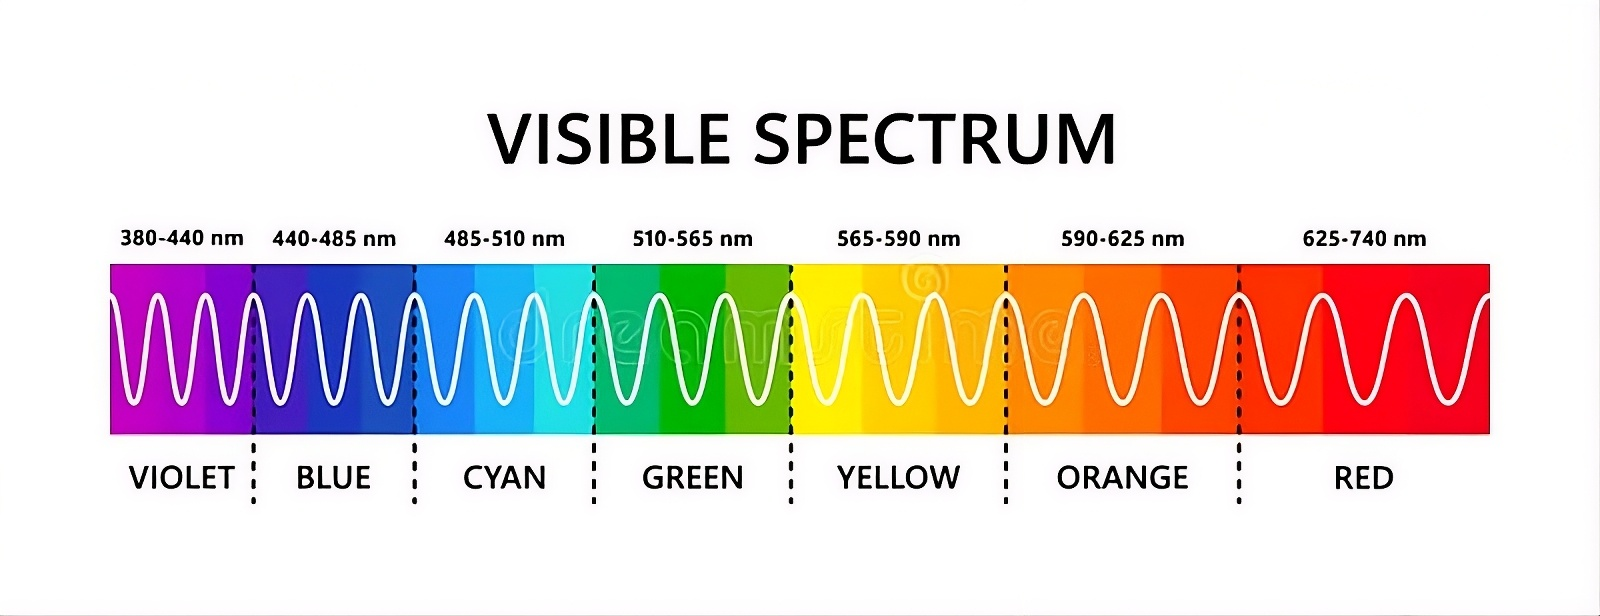
\includegraphics[width=1\textwidth]{images/visible_spectrum.jpg}
                \caption{Espectro eletromagnético.}
            \end{figure}
        \end{column}    

        \begin{column}{0.55\textwidth}
            \textbf{Parâmetros da Colorimetria:}
            \begin{itemize}
                \item Matiz (Hue).
                \item Saturação.
                \item Brilho / Intensidade.
            \end{itemize}
        \end{column}    
    \end{columns}

    \begin{exampleblock}{Aberração Cromática}
        Evitar o uso simultâneo de cores nos extremos opostos do espectro \\(ex: Vermelho Puro + Azul Puro).
    \end{exampleblock}

    \note{
        \begin{columns}[T]
            \begin{column}{0.5\textwidth}
                \scriptsize
                \textbf{Física e Colorimetria:}
                \begin{itemize}
                    \item \textbf{Espectro:} 380 nm (violeta/alta freq) a 750 nm (vermelho/baixa freq).
                    \item \textbf{Matiz (Hue):} Comprimento de onda dominante (o nome da cor).
                    \item \textbf{Saturação:} Pureza da cor (onda pura vs. misturada com luz branca).
                    \item \textbf{Brilho:} Energia luminosa total ($\int$ área sob a curva espectral).
                \end{itemize}
            \end{column}

            \begin{column}{0.5\textwidth}    
                \scriptsize
                \textbf{Aberração Cromática (UI/UX):}
                \begin{itemize}
                    \item \textbf{Refração:} Cristalino dobra cores de forma diferente.
                    \item \textbf{Azul (curta):} Dobra mais, foco à frente.
                    \item \textbf{Vermelho (longa):} Dobra menos, foco ao fundo.
                    \item \textbf{Interface (Pane):} Texto azul em fundo vermelho força o olho a contrair/relaxar o músculo freneticamente para focar no mesmo plano.
                    \item \textbf{Efeito:} Fadiga visual extrema e dor de cabeça em minutos.
                \end{itemize}
            \end{column}
        \end{columns}
    }
\end{frame}